\section{Modeling Cascading Power Failures}

Historically, cascading power failures have been a hard problem to understand, and since they are rare, the process was not studied much.  However, after the Northeast Blackout of 2003, more focus has been devoted to this problem.  

The simplest models of the cascading process are strictly topological models with some mechanism to fail components such as a failed node leads to its neighbors to fail with a given probability.  While these models can capture interesting effects due to degree distribution and clustering, they lack important information about the electrical parameters of the topology as well as loading patterns.   

After discussing historical topological models, Hines, Cotilla. et. al. \cite{hines_2010}, \cite{cotilla_2012} provide a rebuttal to strictly topological models.  Here, topological measures will be looked at in addition to the electrical information behind the topology of the grid. Then, pseudo-topological measures such as electrical distance and centrality will be developed and their importance discussed.

Finally, the Oak Ridge National Laboratory, Power System Engineering Research Center of Wisconsin University, and Alaska University (OPA) type models will be developed.  These models use the electrical parameters as well as demand and generation information to solve the power flow problem.  The results of this are loading patterns on the topology of the power grid.  Using these loading patterns as well as a deterministic or probabilitic failure mechanism, another level of complexity can be added to the cascading failure model.  The following quote from Hines et. al. \cite{hines_2011} supports the use of this type of model.

\begin{quote}
While a perfect model of cascading failure would accurately represent the continuous dynamics of rotating machines, the discrete dynamics associated with relays that disconnect stressed components from the network, the non-linear algebraic equations that govern flows in the network, and the social dynamics of operators working to mitigate the effects of system stress, all power system models simplify these dynamics to some extent. Unlike simple topological metrics, our model does capture the effects of Ohm's and Kirchhoff's laws, by using linear approximations of the non-linear power flow equations \cite{bergen_1986}. Similar models have been used to study cascading failure in a number of recent papers \cite{carreras_2004}, \cite{dobson_2007}, \cite{mei_2009}.
\end{quote}

In addition to the fast time scale cascading model, the OPA work included a slow time scale model, which responded to these cascading failures by engineering improvements.  It is the dynamic interactions of these two forces that leads to an equilibrium in which blackouts of all sizes occur and the size follows a power law distribution.

In order to use OPA models, power flows need to be calculated.  First, the balanced three phase AC power flow equations will be discussed along with its strengths and weakness.  In order to reduce the computational complexity of the model, a Decoupled (DC) power flow model will be developed by making a few simplifying assumptions.

Using the power flow model, an econmic dispatch model can be made to dispatch the generators at least cost, while remaining within its operating constraints.  This dispatch model will be used to connect the reliability issues of the power grid with economic ones.

\subsection{Topologic Model}

This section will first discuss historical topoligical models and then describe common topological measures.  These measures will be used to compare to other network structures.  Using these measures, it is shown that power grids differ from many other common network structures and thus need to be analyzed on there own.  

\subsubsection{Historical Topological Models}

These topological models used flow estimates instead of power flow calculations.

In 2004, Albert et. al. \cite{albert_2004} worked on large blackouts in response to August 2003 and developed a deterministic model of failures based on topological measures.  They used 4 methods of removing nodes from the grid one at a time, randomly, highest degree, highest load, and cascading.  The main simplyfing assumption is that if a generator is connected to a load, its power is available.  In addition, power is routed along the shortest path from generation to load.  Then, in order to monitor the effects of the failure patterns, connectivity loss is recorded, which represent the average decrease in number of generators connected to a substation.  They conclude by noting possible solutions of increasing redundancy and capacity of the system or decreasing reliance on transmission by using more generation at the distrubtion substation level.

Kinney and others developed another method for estimating power flows on a given topology \cite{kinney_2005}.  They introduce the concept of efficiency for power lines and use the harmonic composition of the efficiency of lines to calculate an efficiency measure for any given path.  Now, the electricity is distributed to a load from a generator along the most efficient path.  Then, they modeled an efficiency degradation based on loading through time as well as tolerance measures to outage lines probabilistically.

A handful of these topological models with flow estimates were done in between 2003 and 2010.  Some were predicated on behaving like other networks such as scale-free networks \cite{zhao_2004}, \cite{wang_2009} or small-world networks \cite{ding_2006}.  Others used matching models with a profit function to protect against cascading failures \cite{sun_2008} or novel recourse strategies such as deliberate weak lines for network islanding \cite{duenas-osorio_2009}. 

\subsubsection{Topological Measures}

The topology of a power grid can be described as a unweighted, undirected graph $\cG$ with verticies $\cV$ and edges $\cE \subset (\cV \times \cV)$ which connect the verticies.  A particular grid will be denoted by a subscript, such as $\cG_{EI} = \left\{ \cV_{EI}, \cE_{EI} \right\}$, which would be the graph that represents the Eastern Interconnect.  The verticies $\cV$ on the graph can represent demand nodes, generator nodes, and buses in the transmission network.  The edges $\cE$ represent elements such as transmission lines and transformers.  For convenience, we will define $n_v = \magV$ and $n_e = \magE$.

A useful tool for describing topological measures on graphs is the adjacency matrix, $A$.  The elements $a_{ij}$ of $A$ represent weather nodes $i$ and $j$ are connected, such that if $(i,j) \in \cE$ then $a_{ij} = 1$, else $a_{ij}=0$.  The degree $k_i$ of a node measures how connected it is to the rest of the network, with
\begin{equation}
k_i = \sum_{j=1}^{n_v} a_{ij}
\end{equation}
A common measure to compare different graphs is the average degree $\hat{k} = 2 n_e/n_v$.  Cotilla et. al. \cite{cotilla_2012}, using data for EI from NERC in 2012 and data for WI and TI from FERC in 2005, found the average degree of the networks, which is tabulated in \ref{tab:topo_info}.  This tells us that our power grids are sparsely connected, with around 2.5 transmission elements connecting each vertex, noting that parallel lines are counted as one.  The following statistical analysis of topological measures was done by Cotilla et. al. \cite{cotilla_2012} in order to show that power grids are neither small-world networks nor scale free networks.

\begin{table}
\centering
\begin{tabular}{| c | c c c c c c c|}
\hline
Grid & Verticies & Edges & $\hat{k}$  &  $k_{max}$ & $C$ & $L$ & $d_{max}$ \\
\hline
$\cG_{EI}$	& 41,228	&	52,075	&	2.53	&	29	&	0.068	&	31.9	&	94	\\
$\cG_{WI}$	& 11,432	&	13,734	&	2.4	&	22	&	0.073	&	26.1	&	61	\\
$\cG_{TI}$ 	& 4,513	&	5,532		&	2.45	&	18	&	0.031	&	14.9	&	37	\\
\hline
\end{tabular}
\caption{Topological measures for the three US power grids}
\label{tab:topo_info}
\end{table}


There are many statistical measures used to compare our power grid graphs to other common graph structure.  The first measure is the distribution of the degree, $k_i$, of all the nodes.  One type of network to compare to is a scale-free network which have a power-law degree distribution.  These networks have highly connected central hubs, which are inherent weak points to the network.  However, high-degree nodes are far less common in power grids than would be expected with a scale-free network.    

Two additional measures, which are distance metrics, are diameter and characteristic path length.  The distance $d_{ij}$ between $i$ and $j$ is the minimum number of links needed to traverse from vertex $i$ to vertex $j$.  The diameter is then 
\begin{equation}
d_{max} = \max_{ij} d_{ij}
\end{equation}
 and the characteristic path length is 
\begin{equation}
L = \frac{1}{n_v (n_v -1)} \sum_{\forall i,j | i \neq j} d_{ij}
\end{equation}
In addition, the average nodal distance $\hat{d} = \sum_{j=1}^{n_v} d_{ij}$ can be used.  As the size of small-world networks increase, the characteristic path length increases roughly with $\ln n_v$, which means the distances between verticies grows slowly.  However, the power grid's path length always grows faster than $\ln n_v$ and falls between small-world networks and regular grids, which scale linearly with $n_v$.

Another useful measure will be the cluster coefficient which gives insight into neighborhoods of nodes.  Let $e_i$ be the number of edges connected to vertex $i$ and its immediate neighbors $N_i$ by the following $e_i =\sum_{\forall j,k \in \left\{ N_i \cup i \right\}} a_{jk}/2$.  Then the clustering of node $i$ is
\begin{equation}
c_i = \frac{e_i}{(k_i(k_i-1))/2}
\end{equation}
and the cluster coefficient of the graph is $C = \frac{1}{n} \sum_{i=1}^{n_v} c_i$.  Power networks were found to have less clustering then small world networks but much larger than random grids, which may be due relatively few long distance lines.

The final measure used was degree assortativity, which is the correlation of the degree of two connected nodes.  Power networks were found to have small, negative degree asortativity.  This was due to distribution feeders, which have a large number of radial lines connecting single loads to the substation.  This behavior was not found in small-world networks.

Hines et. al. \cite{hines_2010} conclude that while these topological measures are useful for understanding the structure and perhaps indicating general vulnerabilities, they can lead to erroneous conclusions.  For example, Kinney et. al. \cite{kinney_2005} and Albert et. al. \cite{albert_2004} draw different conclusions about such things as the effects of single outages using similar data.  Power flow based models are more realistic and thus more useful for vulnerability analysis.  However, these measures are similar to electrical topological measures that will be discussed later and can be very useful.



\subsection{OPA Model}

The next level of complexity to add is to use electrical information about the grid as well as loading patterns to determine the power flows.  The loadings on particular elements have a large effect on the failure probability of the given element.  This type of model was done by three groups, Oak Ridge National Laboratory, Power System Engineering Research Center of Wisconsin University, and Alaska University.  This class of models will be called OPA models.  They look at the power transmission system and consider engineering and physical aspects, as well as economic, regulatory, and political responses to balckouts and increases in load.

In 2001, Dobson et. al \cite{dobson_2001} found that the opposition of the slow time scale force of growth in load and system capacity and fast time scale of cascading power failures and outages produced a dynamic equillibrium that can be seen in real world data.  Many real world complex systems can be seen to have this self-organized criticality property.  This criticality means that the blackout size distribution follows a power-law distribution, $f(x) = ax^k$ with an exponent of $-1.3 \pm 0.2$,  making large blackouts more likely.  In addition to criticality, it also appear to be in an equilibrium.  The distribution of blackout size has not changed in the past 30 years.  They argue that you can't study larges blackouts by looking at initial triggering events only, but you must look at the root cause, and deeper, long-term forces that drive the evolution of power system.

On a slow time scale, there are several things that happen to the electricity grid.  The first main force is the slow growth in load (around 0.7\% growth per year for first decade of 21st century \cite{eia_gov}).  This has the effect of reducing the available capacity margins on power lines and increasing the likelihood of failures as well as possibly further constraining economic dispatch.  While the slow time scale is progressing, random exogenous events, acts of nature, happen to outage individual components.  These possibly initiate large cascading failures and blackout portions of the system.  The engineering response to blackouts in operating policies, maintenance, equipment and controls have the effect of increasing margins on the slow time scale.  These forces push against each other and settle in an equillibrium.

The following parts go through the details of these forces mathematically.  These are drawn from several OPA papers \cite{dobson_2001}, \cite{carreras_2004},\cite{dobson_2007}.  

\subsubsection{Slow Time Scale}
The slow time scale is simplified by using days as the time step, represented by index $t$.  There are three main components to the slow dynamics.
\begin{enumerate}
\item The demand grows at the beginning of each day.  We have $d_{it} = \lambda d_{i \rho(t)}$ where $\rho(t)$ represents the preceding time period and $i$ is a vertex with a load demanding $d_{it}$ on day $t$ at peak load.  They used $\lambda = 1.00005$, which corresponds to a yearly growth rate of $1.8\%$ (the yearly average for 1980-2000).  To represent daily load fluctuations, all loads are multiplied by a random number $r$, such that $2-\gamma \le r \le \gamma$ with $1 \le \gamma \le 2$.
\item The response to blackouts is to upgrade the transmission system by increasing the maximum capacity of transmission lines.  If a line has overloaded in a blackout, the response is to increase its capacity so that $U_{et} = \mu U_{e \rho(t)}$ with $e$ being an edge with capacity $U_{et}$ on day t.  They varied $\mu$ between $1.01$ and  $1.1$.  This parameter simplifies all of the efforts that go into these responses including increasing the frequency of maintenance, changing operating policy, installing new equipment, and adjusting or adding alarms and controls.  These responses are modeled as happening before the next day, but in reality can take place over many different time scales.
\item The response to increased demand is to increase generator power so that all demand can be met.  First, they assume that increases in power is quantized and not continuous.  The quantity $\Delta G_t = \kappa ( D_t / n_g )$ represents the amount of power increase for a generator with $\kappa$ being a few percent, $n_g$ being the number of generators, and $D_t = \sum_{i \in \cV} d_{it}$ is the total demand for time period $t$.  In order to increase generation at a node $i$, we need $g_{it}^+ + \Delta G_t \le \sum_{e=(i,j) | e \in \cE} U_{et}$, that is, the increased power needs to be able to flow out of its neighborhood.  $g_{it}^+$ represents the maximum power generation at node $i$ on day $t$.  Power is continued to be added to eligible nodes, $g_{it}^+ \leftarrow g_{it}^ + + \Delta G_t$, until the generator capacity margin has risen above a prescribed level.  The generator capacity margin is defined by
\begin{equation}
\left(\frac{G-D}{D}\right)_t = \frac{\sum_i g_{it}^+ - D_0 e^{(\lambda-1)t} }{D_0 e^{(\lambda-1)t}}
\end{equation}
with $D_0 e^{(\lambda-1)t}$ being the average power demanded not including daily fluctuations.  The generator capacity margin is used to deal with daily fluctuations in demand.  The generator capacity margin of the U.S. has an estimated mean value between 15\% and 30\% \cite{carreras_2004}.
\end{enumerate}

These forces balance against system outages throughout time.  The outages were modeled as being possible to take place every day and begin with random events with a given probability.  The next section will go into detail about the cascading process that is possible after the random events take place.

\subsubsection{Fast Time Scale}

Individual blackouts triggered by random events (equipment failure, weather, vandalism, attack) can become widespread through a series of cascades. 
The initial goal of building this cascading failure model was to produce a list of lines that could plausibly be involved in cascading event.  It simplifies the process of cascading failures considerable but is still able to capture important effects of topology changes throughout the process.  Figure \ref{fig:cascade} gives a quick overview of the fast time scale simulation used to model cascading power failures.

\begin{figure}
\centering
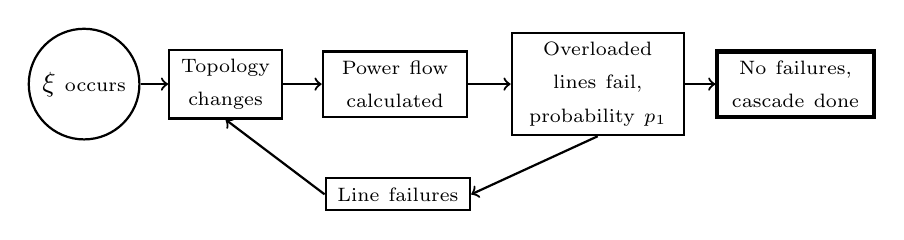
\begin{tikzpicture}
\draw [->,thick] (1,1) node[anchor=east, circle, draw]{$\xi$ \scriptsize occurs}
-- (1.35,1) node(TC)[anchor=west,text width=1.2cm,text centered,  rectangle, draw]{\scriptsize Topology changes};
\draw[->,thick] (TC)
--(3.3,1) node(PF)[anchor=west,text width=1.6cm,text centered, rectangle,draw]{\scriptsize Power flow calculated};
\draw[->,thick] (PF)
--(5.7,1) node(F)[anchor=west,text width=1.95cm, text centered, rectangle, draw]{\scriptsize Overloaded lines fail, probability $p_1$};
\draw[->,thick] (F)
--(8.3,1) node(DN)[anchor=west,text width=1.75cm, text centered,rectangle,draw,line width=1.5pt]{\scriptsize No failures, cascade done};
\draw[->,thick] (F.south)
--(5.2,-.4) node(LF)[anchor=east,text width=1.6cm, text centered, rectangle, draw]{\scriptsize Line failures };
\draw[->,thick] (LF.west)
-- (TC.south);

\end{tikzpicture} 
\caption{OPA simulation of a cascading power failure}
  \label{fig:cascade}
\end{figure}


The OPA model of the cascade process begins with an exogenous event, $\xi$, that effects the topology of the grid.  In their initial version, $\xi$ were the branches that randomly failed in an independent and identically distributed (I.I.D) manner, a Bernoulli trial with probability $p_0$.  Moments after the outage, the power flows are rerouted through the new topology based on the laws of physics.  In a longer time frame, it is possible for operators to take actions such as load shed and generator redispatch.  The resulting loading on the transmission lines is evaluated.  Their model then failed overloaded transmission lines with a Bernoulli trial with probability $p_1$ between  0.1 and 1.  After all overloaded lines are tried, a transition is made to the next stage.  Either there are no more outages, in which case the cascade is over, or more branch elements are outaged, the topology changes, and the operator is allowed to take recourse.  This process repeats until the system is stable and no outages occur.  Figure \ref{fig:cascade-example} shows a visual example of the cascading process.

For a given grid $\cG$ and initial demand $d_0$
\begin{description}
\item[ Initial $ \xi $ ]  For $e=1,...,n_e$, draw $\omega$ from $U[0,1]$ and if $\omega \le p_0$, line $e$ is outaged.
\item[ ] \hspace{35px} \vdots 
\item[ Stage $m$ ]  Calculate the power flows $f_{m}$, a column containing the branch flows for all edges in $\cE$, by using DC power flow equations with demand vector $d_m$. 

For $e=1,...,n_e$, if branch flow $f_{em} \ge U_{em}$, draw $\omega$ from $U[0,1]]$ and if $\omega \le p_1$, outage line $e$.
\end{description}

\input{cascade_example}

\subsubsection{Dynamic Equillibrium}

These opposing forces eventually find an equillibrium.  The equillibrium tends to be near critical points, which are points that have maximum power flow through the network for the nominal system capacity.  The system self-organizes towards these points which maximize efficiency of its assets.  When the system approaches these critical points, the power flow becomes limited due to two possible causes. 
\begin{itemize}
\item The power flows are limited due to tranmission line constraints.  This type of critical point has larger blackouts but happen less frequently.  In addition, the blackouts typically have  multiple lines tripping.
\item The power flows are limited due to generation capacity.  This results in frequent blackouts but of smaller size.
\end{itemize}
However, it is also possible to be in an operating regime which is close to both types of critical points simultaneously.  When this is the case, blackouts of all sizes occur.  While this operating regime may not be good from a reliability standpoint, it has the desirable characteristic of being able to deliver the maximum power for the system.   That is, when these two points are balanced, the system is capable of maximum throughput from its generators to its loads with minimal excess capacity.  This is important from an economic perspective and a critical reason the system self-organizes to these types of points.  This type of point tends to be the cheapest way to supply all the loads with power, while statisfying the minimum system reliability standards.

\subsubsection{Additional Complexities}

The OPA model can be extended to include additional complexities for many different reasons.  It is always a balance of how much resources you have to solve the problem and the amount of resolution you need in the solution.  The base OPA model is easy and fast to replicate, however by trying to gain increased resolution in the output, the model becomes increasingly complex and difficult to solve in a timely manner.

In related work, Chen et. al. \cite{chen_2005} find many similar conclusions to the OPA model by using an extension which included a hidden failure model.  A hidden failure is undectable in normal operations, but as the system becomes disturbed, a relay may incorrectly trip.  These protective relays are in operation to protect the line from overloads and disconnect it from the system.  This work introduces a loading dependent failure model that trips neighboring lines to outaged components.  This hidden failure is exposed the first time a disturbence nearby occurs and if it doesn't fail then, it is assumed to be properly operating and future disturbances will not undergo this hidden failure mechanism.  The probability of these happen in the real world are non-negligble according to NERC data \cite{nerc_dawg}.  

This work displays many similar results to the OPA papers.  First, the power law behavior near critical loading can be seen by varying the system loading levels.  They find that by increasing spinning reserves the risk of big blackouts is greatly reduced.  The blackout size distribution tends towards an exponential distrubition as reserve levels are increased.  By lowering the hidden failure rate, the system becomes more robust and larger blackouts become less likely.  Finally, they note that prompt control actions can reduce the risk of big disturbances.  While all of these results seem fairly straightforward, it points to the fact that the important aspects of the cascading process are being modeled and the effects are similar to what would happen in the real world.

Bienstock made several modifications \cite{bienstock_2011} to the original OPA model in order to remove some undesirable effects of the simulation, notably the erratic behavior of its output under small changes in the input.  To do this, he introduced the concept of memory to the system.  In order to see if a line is in or near an overloaded state, it uses a running time average of the current state and previous states.
\begin{equation}
\tilde{f}_{et} = \alpha f_{et} + (1-\alpha) \tilde{f}_{e\rho(t)}
\end{equation} 
Here, $f_{et}$ represents the power flow on edge $e$ at time $t$.  Then, $\tilde{f}_{et}$ is used in the overload and outage calculations.

In addition to including a memory, he also smoothed out the definition of an overloaded line by creating a step in between normal and overloaded states in which the failure probability was more than nominal but less than in the overloaded state.  Using $0 \le \epsilon \le 1$, for edge $e$, the following failure model smooths the effects of overloaded lines failing.
\begin{align}
\tilde{f}_{et} \ge (1+\epsilon) U_{et}			&	\hspace{10pt} \mbox{The line outages with certainty} 	\\
(1-\epsilon) U_{et} < \tilde{f}_{et} < (1+\epsilon) U_{et}	&	\hspace{10pt} \mbox{The line outages with probability }\frac{1}{2} 	\\
\tilde{f}_{et} \le (1-\epsilon) U_{et}			&	\hspace{10pt} \mbox{The line remains in operation} 
\end{align}

An AC power blackout model was developed at the University of Manchester (Manchester Model) by Nedic \cite{nedic_2006} and the original OPA authors.  This model is able to represent real world disturbances more accurately by using the full non-linear model that describes power flow.  This gives resolution into areas for generator instability, under-frequency load shedding, redispatch of active and reactive sources, and emergency load shedding.  The model has both automated control systems and operator recourse.  This model was used in OPA criticality works by Mei et. al. \cite{mei_2006}, including one with mechanisms using voltage stability margins \cite{mei_2008}.  However, the additional complexity comes at the cost of having to solve a nonlinear program and the loss of convergence gaureentees.  This is all done in order to represent something that is a companion too, but not the main driver of the cascading process (according to the Northeast outage working group, the main driver was angle instability not voltage instability).

Mei and others have worked to improve the accuracy of OPA by increasing the amount of details modeled \cite{mei_2009}.  In the fast dynamics, along with protective relays being modeled as hidden failures, they included a failure mechanism for the operational dispatch center that is responsible for generator redispatch.  In addition, they used a failure model where an underloaded line is failed with probability $p_1 \left( f_e/U_e \right)^N$, with $N=10$.  For the slow dynamics, they added a step that models a planning department by increasing the capacity of lines which have a loading rate $\left( f_{e}/ U_{e}  \right)$ greater than a set point.  

In 2013, Qi et. al. extended this model to include slow dynamics of vegetation growth and management.  Neglecting spatial variation and heating/cooling effects from   the environment, they model line temperature by a differential equation
\begin{equation}
\frac{dT(t)}{dt} = \alpha I^2 - \nu (T(t) - T_0)
\end{equation}
where $T(t)$ is the line temperature at $t$, $I$ current, $T_0$ initial temperature, and $\alpha$ and $\nu$ are calculated parameters.  This can be solved by assuming constant branch flow, $f$, to calculate the temperature over time
\begin{equation}
T(t) = e^{-\nu t}\left( T_0 - T_e(f) \right) + T_e(f)
\end{equation}
which can be used to find the final equilibrium temperature, $T_e(f)$ (a function of its constant power flow $f$ on the line), and time until a given temperature.  Using the calculated temperature, the horizontal span, and an elongation parameter, the line sag distance can be calculated.  When the minimum distance between lines and vegation passes a breakpoint based on transmission line characterestics such as operational voltage, the line will be outaged.  They model the vegetation with a daily growth rate model and include a managment simulation in which they identify future potential hazards and cut down trees over time.  The statistical analysis of there model aggreed well with historical data in China.



\subsection{Power Flow}
In order to run the OPA simulation of cascading failures, the ability to calculate power flows on the system is critical.  To model a balanced, three phase power flows, in full resolution we need to use the concept of complex power.  The alternating current of the power system can be represented by sine or cosine waves.  A three phase power system has three lines for each transmission element and each line has a wave that is out of phase with the other two.  Using one wave as a reference, the other phases will attempt to be 120 degrees behind reference and 120 degrees ahead of refrence.  This improves the efficiency and quality of power for loads over a 2 line system as well as not requiring an excessive amount of lines for each transmission element.  

After going into details about complex power and electrical parameters of transmission elements, the balanced three phase power flow equations will be shown.  These non-linear equations model the net power and reactive power injects as well as voltage and phase angle at each vertex of the power system.  A few simplifying assumptions will be made to allow the equations to become linear for the DC (decoupled) power flow equations.  Then, using the dc power flow model, basic economic dispatch and unit commitment models will be shown.  Finally, some pseudo-topological measures will be reviewed that will be useful in the optimization process.

\subsubsection{Electrical Information}
Complex power has both real and reactive parts.  Alternating currents  on a circuit affect components of energy storage such as inductors (changing the current is opposed by a voltage)  or capacitors (store electrical charge).  Over one full cycle of the electricity changing direction, across any individual element there can be real power transfered.  However, there is also power which is stored and released within one cycle and the net energy transfer of this power is 0.  This is called reactive power and is modelled as the imaginary component of complex power.  Let $S_i$ be the complex power inject at some bus on the grid, that is
\begin{equation}
S_i = P_i + j Q_i = V_i I_i^*
\end{equation}
where $P$ is real power, $Q$ is reactive power, $V_i$ is complex voltage, and $I_i^*$ is the complex conjugate of current.  
	
To model a transmission line, the characteristic impedence is used.  At any point, there is complex current I, in each individual line in the transmission element.  Also, there is a complex voltage V difference between the lines.  The characteristic impedence (generalization of Ohm's Law) is then
\begin{equation} \label{impedence}
V/I = Z_0
\end{equation}

Here is a phasor representation of complex voltage $V_i = | V_i | e^{i (\omega t + \delta_i) }$, where the real voltage would be Re[$V_i$]$=\cos (\omega t + \delta_i)$.  Now, by modeling \ref{impedence} in phasor notation, we have 
\begin{equation}
 | V_i | e^{j (\omega t + \delta_V) } = | I_i | e^{j (\omega t + \delta_I) }  | Z_i | e^{j ( \delta_Z) } = |I||Z|e^{j (\omega t + \delta_I + \delta_Z)}
\end{equation}
For this equation to hold at all times $t$, we know that this must hold $\delta_V = \delta_I + \delta_Z$.  When an element has $\delta_Z = 0$, the current and voltage are exactly in phase and it is a purely resistive load with no reactive production or absorption. 

The lines can be modelled using a pi model (schematic diagram looks like $\pi$), which uses line parameters of resistance $R$, inductance $L$, conductance $G$, and capacitance $C$. 
\begin{equation}
Z_0 = \sqrt{  \frac{R+j \omega L}{G+j\omega C} }
\end{equation}
The system angular frequency is $\omega = 2 \pi f$, where $f$ is frequency here.  

If a transmission element is loaded at its surge impedence loading, it neither creates nor consumes reactive power.  This level is defined by 
\begin{equation}
SIL = V_{LL}^2 / Z_0
\end{equation}
Where $V_{LL}$ is the line to line voltage.  When a transmission line is at a level below this, it will supply reactive power and raise system voltages.  When the loading is above this level, the transmission line consumes reactive power, depressing voltages.

\subsubsection{Balanced Three Phase Power Flow}
In a balanced three phase system, at every vertex $i$, we have
\begin{equation}
S_i = P_i + j Q_i = V_i I_i^*
\end{equation}
In addition, with $KCL$, we have $I_i = \sum_{k=1}^n Y_{ik} V_k$, where $Y$ is the admittance bus matrix.  The admittance is the inverse of imdedence, that is
\begin{equation}
Y = G + j B = 1/Z = 1/(R + jX) 
\end{equation}
where $B$, the imaginary part of admittance, is susceptance and $X$, the imaginary part of impedence, is reactance.  Now we have that the complex power at every vertex $i$ is
\begin{equation}
S_i^* = P_i - j Q_i = V_i^* \sum_{k=1}^n Y_{ik} V_k
\end{equation}
By converting these into rectangular coordinates, we get two equations for each bus
\begin{align} \label{ac-pf}
P_i = \sum_{k=1}^n |V_i| |V_k| \left[ G_{ik} \cos (\delta_i - \delta_k) + B_{ik} \sin (\delta_i - \delta_k) \right]  \\
Q_i = \sum_{k=1}^n |V_i| |V_k| \left[ G_{ik} \sin (\delta_i - \delta_k) - B_{ik} \cos (\delta_i - \delta_k) \right]  
\end{align}

For each bus, in addition to $P_i$ and $Q_i$,  we have its voltage $|V_i|$ and its phase angle $\delta_i$.  So, we have $4 n_v$ variables and $2 n_v$ equations.  By supplying the value to $2 n_v$ variables and defining a slack bus, we can find unique values for the remaining $2n_v - 1 $ variables.  Depending on the type of bus, different variables are supplied.  If it is a generator, both $P$  and $V$ are supplied.  A load is defined by a $P$ and $Q$.  The slack bus is a generator in which the phase angle is set to 0.  The phase angle $\delta$ and reactive power production $Q$ are found for each generator and the phase angle $\delta$ and the voltage $|V|$ are found for the loads.

\subsubsection{Decoupled Power Flow}
This model makes assumptions such as lossless lines, small voltage angle differences, and a flat voltage profile.  This is a common simplifing model which is used routinely in economic and reliability analysis of power systems.  A flat voltage profile implies that $\forall i \in \cV$, we have $V_i = 1$.  Small voltage angle difference in conjunction with sine and cosine give the following approximations
\begin{align}
\cos(\delta_i - \delta_j) &\approx 1	\\
\sin(\delta_i-\delta_j) & \approx \delta_i - \delta_j
\end{align}
In addition, since these lines are lossless, $R$ and $G$ are 0.  

The following equations represent the necessary constraints on the power flow in this lossless system.  The first equation represents the conservation of energy and the second equation represents Kirchoffs Current Law.  Conservation of energy implies that the sum of generation and demand is equal to 0 at every point in time.
\begin{align}	\displaystyle
\sum_{j | e=(i,j),  e \in \cE}{f_{e}} &= g_{i} -d_{i} \hspace{17px}   \forall i \in \cV   \label{pf1}
\\
\theta_{i} - \theta_{j} &= X_{e} f_{e}			\hspace{27px}	\forall e=(i,j) \mbox{ s.t. } e \in \cE   \label{pf2}
\end{align}
The value $p_{i} = g_{i} - d_{i}$ represents the net power inject for that node.  A reliability focused model would seek to maximize demand served at all points in time.

When a line is outaged, the power flow has obviously dropped to 0, that is $f_e = 0$.  In addition, the constraint \ref{pf2} to the system is no longer there and must be removed from the formulation.

\subsubsection{Economic Dispatch}
To clear the electricity market at a single point in time, a least cost dispatch model is used.  This model takes bids from generators, a known demand, as well as transmission and ramping constraints and finds a set of generator outputs which meet the demand at least cost.  Using a quadratic cost function for the generators (this cost function can be thought of as a bid from generators which includes the profit the generator would like to make for each marginal unit of production), the least cost dispatch model is as follows. 

The following model is a quadratic program with linear constraints.  The objective function is to minimize the cost of generation.  Typical least cost dispatch and unit commitment models will make various assumptions to allow for linear constraints versus the physical nonlinear constraints to which the power system is subject.  This is the most basic least cost dispatch model, which could be used for clearing the real-time market.  Models in use can have extensions such as ''$N-1$ constraints", which are reliability and security requirements.

\begin{subequations}
\begin{align}
 \min \sum_i \alpha_i g_i &+ \beta_i g_i^2	+ W_i(\tilde{d} - d_i)&	\\
g_i - d_i &= \sum_j f_{ij}	&	\forall i \in N 	\\
X_{ij} f_{ij} &= \delta_i - \delta_j & \forall (i,j) \in M \\
g_i  &\in \left[ g_i^- , g_i^+ \right]		&	\forall i \in N 	\\
f_{ij} &\in \left[ -U_{ij}, U_{ij} \right]	&	\forall (i,j) \in M 
\end{align}
\label{leastcostdispatch}
\end{subequations}

Here, $\alpha_i g_i + \beta_i g_i^2$ can be seen as the cost function for the generator at node $i$ and $W_i(\tilde{d} - d_i)$ is the cost for shedding load.  The generator is bounded between a maximum $g_i^+$ and minimum $g_i^-$ that represent its ramping rate over a specific time interval.  

The day-ahead market uses unit commitment models.  This model will have power flow equations for each $t \in \cT$.  These are integer programs due to the introduction of binary variables $y_{it}$, which take on the value 1 if the generator is switch on and 0 if the generator is off.  The following logical constraint enforces this by
\begin{equation}
y_{it} g_i^- \le g_{it} \le y_{it} g_i^+
\end{equation}
The cost function can then include a fixed cost for operating a generator, such as increased staff during operation.  This cost is not dependent on the level of production but rather if the plant is in an on or off state.  The cost function for each node $i$ and time period $t$ is
\begin{equation}
\alpha_i g_it + \beta_i g_{it}^2 + c_i y_{it}
\end{equation}
This subproblem will be used in a full day model in which the power flow problem is solved for each time period, while remaining feasible with respect to ramping rates and on and off times for generators.



\subsubsection{Pseudo-Topological Measures}
Cotilla et. al. \cite{cotilla_2012} use the fact that voltage phase angles between areas as measure of stress in power networks (47).  Using the power flow Jacobian matricies,
\begin{equation}
 \Delta P = \frac{ \partial P }{ \partial \theta} \Delta \theta + \frac{ \partial P }{ \partial | V | } \Delta | V |
\end{equation}
and assuming voltages are held constant, then $\frac{ \partial P }{ \partial \theta} $ is a Laplacian matrix.
Set the conductance matrix $G = \frac{ \partial P }{ \partial \theta}$, then with
\begin{equation}
e_{ij} = g_{ii}^{-1} + g_{jj}^{-1} - g_{ij}^{-1} - g_{ji}^{-1}
\end{equation}
$E$ satisfies properties of distance matrix under dc power flow assumption, and empiraclly held otherwise.  $E$ is weighted and fully connected with $n_v(n_v-1)$ links.

We then have a quantity that is analogous to node degree, $k_i$, called electrical distance
\begin{equation}
e_i = \sum_{j=1}^n \frac{e_{ij}}{n-1}
\end{equation}
with the inverse representing centrality
\begin{equation}
c_i = e_i^{-1}
\end{equation}

A unweighted graph can represent these distances.  Let $R$ be an adjencency matrix and by defining $r_{ij} = 1 $ if $e_{ij} < t$ and adjusting $t$ so that there are  $n_e$ links.  $R$ has lots of nodes with no connection, with the interpretation that few nodes have disproportionate influence on a large portion of the nework.

Comparing the topological and electrical measures, Cotilla et. al. \cite{cotilla_2012} have that the topological distances have exponential tail and the electrical distances have power-law tails.  Also, there is weak correlation between the two types of distances.  Electrical centrality seem to point out very well the importance of each node to grid stability.  This may be used to find areas to improve the network.

\subsection{Design Problems}
These are examples of design problems, which would aim to make the system more robust for a given budget.

\subsubsection{Transmission Expansion}
Add or expand capacity on transmission system

\subsubsection{Vegetation Management}
Find important areas to be extra vigilent with vegetation practices
\cite{qi_2013}

\subsubsection{Allocating Reserves}

REGULATION AND RESERVES

In this case an operating configuration need not be given.  The program can either search for an operating configuration as well as reserves or given an operating configuration, allocate the reserves.  These operating reserves determine where the system is able to relieve congestion in a contingency.

\subsubsection{Generator Redispatch}
This model tries to find a operating configuration that is within a given distance from the current operating regime and minimizes the worst case scenario outage.  The input for this model is the current operating configuration $(p_0, d_0)$ as well as a distance vector $\delta$ that represents how far each generator can move from its current output levels.  In this case, the root node of the stochastic tree will have variables that represent initial generator output levels and the child trees will be constrained from how far they can move from this.  Also, a continuous variable will be added that represents the amount of load shed in the worst case scenario.  The objective will be to minimize the load shed in the worst case scenario.  
This program could be used when the system is becoming close to unstable and cost concernes become less of a priority than system stability.

\subsubsection{Energy Storage}
The ability to store energy and dispatch it creates an arbitrage opportunity on the time-varying price of electricity.  Arbitrage is the process of taking advantage of price differences in different markets.  Here, the different markets are simply the points in time during the day, at which each point must have a supply of electricity greater than demand.  The demand for electricity has both daily and seasonal variation.  The price of electricity tends to be low during the night and winter and high during the day and particularly summer.  To engage in arbitrage over the daily variation of electricity prices, one would store energy during the night when the prices are low and then sell during the day when the prices are high.  

TYPES OF ENERGY STORAGE

Chemical, Thermal, Electrical, Momentum

There are two forms of arbitrage availble based on the electricity markets.  The first type is a risk-free arbitrage that earns a profit and no possibility of negative cash flows by operating strictly on the day-ahead market.  The other type is a statistical arbitrage which utilizes the day-ahead and real-time market and refers to a positive expected profit.    

The operation and placement of these devices could be done in such a way as to improve the reliability of the system.  Since we know that outages are more likely near stressed points, by reducing the volatility of the system, we will have lowered peak loadings and be moving away from critical points.




